
\chapter{Methods}

\label{chap:methods}

\section{Molecular dynamics}
\label{sec:th_md}

Molecular dynamics simulations are a powerful tool for modeling the vibrational energy transfer in atomic scale systems. In MD, the classical Newton's equations of motion \eqref{eq:th_eom} [or more generally the Langevin equation \eqref{eq:th_ohmic} for atoms coupled to heat baths] are integrated numerically. The forces $\bb{F}_i$ are calculated from an analytical expression obtained from the interatomic potential function $\ca{V}$ as $\bb{F}=-\partial \ca{V}/\partial \bb{r}_i$ and therefore include all orders of anharmonic terms. By simulating the steady-state non-equilibrium for sufficiently long times, one can extract values of macroscopic observables such as the heat current accurately by time-averaging. Based on the ergodicity principle, the time averages are expected to equal the statistical average over the corresponding ensemble. In the following, we briefly go through the most important aspects related to a MD simulation.

% One key aspect of the method is the assumption of ergodicity: statistical ensemble average can be calculated from a time average, meaning that  %In a microcanonical simulation, for example, the system should sample all the states that lie on the constant-energy manifold determined by the initial conditions. 

In MD, the equations of motion are integrated numerically using a finite-difference method. The pool of the finite-difference methods includes, e.g., Euler methods, Verlet methods, Runge-Kutta methods, the leap-frog method and predictor-corrector methods \cite{allentildesley}. In all the simulations of this work, the velocity Verlet algorithm was employed to integrate the equations of motion. While velocity Verlet exhibits moderate short-term energy drift, it is very simple to implement, efficient and it possesses very small long-term energy drift due to its being both time-reversible and symplectic \cite{frenkelsmit}. The velocity Verlet update equations for the positions $\bb{r}_i$ and velocities $\bb{v}_i=\dot{\bb{r}}_i$ are \cite{allentildesley}
\begin{alignat}{2}
  \bb{r}_i(t+\Delta t) &= \bb{r}_i(t) + \bb{v}_i(t)\Delta t+  \frac{1}{2}\bb{a}_i(t) \Delta t^2 + \mathrm{O}(\Delta t^4) \\
  \bb{v}_i(t+\Delta t) &= \bb{v}_i(t) + \frac{ \bb{a}_i(t)+\bb{a}_i(t+\Delta t)}{2} \Delta t+ \mathrm{O}(\Delta t^2) ,
\end{alignat}
where $\Delta t$ is the time step and $\bb{a}_i(t)=\bb{F}_i(t)/m_i$ is the acceleration.

To outline the typical steps involved in a non-equilibrium simulation, consider the example setup of Fig. \ref{fig:intro_systems}(b) used to investigate the anharmonic effects in interfacial heat transfer. First the whole structure is equilibrated by running a zero-pressure simulation at prescribed temperature using a combination of a Nos\'e-Hoover barostat and thermostat, allowing the structure to conform to zero-stress state. Typical equilibration period consists of a few hundreds of thousands of time steps. After the initial equilibration, the size of the simulation box is fixed, as are atoms located at the left- and right-most unit cells in the system. This prevents atomic sublimation at the free surfaces. Particles in the ''hot'' and ''cold'' regions, illustrated by the red and cyan coloured atoms in Fig. \ref{fig:intro_systems}(b), are coupled to heat baths at temperatures $T_{\textrm{hot}}$ and $T_{\textrm{cold}}$. The system is then allowed to reach non-equilibrium steady state by running MD until the temperature profile and the heat current flowing through the system fluctuate around constant values. After this initial period, simulation is continued typically for millions of time steps, and the values of the observables of interest are collected from the run. The statistical error in the collected observables can be estimated by using standard methods described, e.g., in \citepub{fpu}.


%\textbf{SIMULATION FLOW}

\subsubsection{Lattice heat current}
\label{sec:spectral}
The main observable of interest in heat transfer simulations is the heat current flowing through system, which can be expressed as a sum of interatomic heat currents flowing across a specified cross-section of the simulation domain. The expression for the interatomic heat current can be determined by calculating the temporal rate of change in the local energy consisting of kinetic and potential energy contributions \cite{hardy63,lepri03}. For the average heat current flowing from atom $j$ to atom $i$ one thereby gets (see \citepub{fpu} for derivation) 
\begin{equation}
 Q_{j\to i} = \left\langle \frac{1}{2} \bb{F}_{ij} \cdot \left( \bb{v}_i+\bb{v}_j \right) \right\rangle, \label{eq:th_Qji}
\end{equation}
where the force acting on atom $i$ due to the interaction with atom $j$ is obtained from the pairwise potential energy $V_{ij}$ as
\begin{equation}
 \bb{F}_{ij} = - \frac{\partial V_{ij}}{\partial \bb{r}_i}.
\end{equation}
The angular brackets in Eq. \eqref{eq:th_Qji} denote non-equilibrium ensemble average, which can be calculated by time-averaging in MD simulations. 

Equation \eqref{eq:th_Qji} cannot directly indicate, which vibrational frequencies are actually responsible for the energy transfer. Such an analysis was enabled in \citepub{spectral}, where an expression for the spectral decomposition $q_{j\to i}(\omega)$ of heat current was derived. The decomposition is defined implicitly through the formula
\begin{equation}
 Q_{j\to i} = \int_0^{\infty} \frac{d\omega}{2\pi} q_{j\to i}(\omega)
\end{equation}
and was shown to be given by the expression
\begin{equation}
 q_{j \to i}(\omega) = 2\textrm{Re} [\tilde K_{ij}(\omega)],
\end{equation}
where $\tilde K_{ij}(\omega)=\int_{-\infty}^{\infty} dt e^{i\omega t}K_{ij}(t)$ is the Fourier transform of the time-domain correlation function
\begin{equation}
 K_{ij}(t_1-t_2) = \frac{1}{2} \left\langle \bb{F}_{ij}(t_1) \cdot \left[ \bb{v}_i(t_2)+\bb{v}_j(t_2)\right] \right\rangle \label{eq:th_Kijt1t2}
\end{equation}
The force-velocity correlation function depends explicitly only on the time-difference $t_1-t_2$ due to the assumed steady-state. 

The correlation function can be calculated by analyzing the force and velocity trajectories obtained from non-equilibrium molecular dynamics simulation. In practice, it is useful expand the interatomic force $\bb{F}_{ij}$ in terms of small displacements from equilibrium positions, allowing for simplifying the post-processing and detailing the relative contributions of linear and non-linear energy transfer mechanisms. The contributions of non-linear terms to the interfacial thermal conductance were analyzed in \citepub{spectral}. In \citepub{cnt}, only the dominant linear term was included in investigating the phonon transmission in carbon nanotubes.





\section{Green's function methods}


\subsection{Self-consistent heat bath model}
\label{sec:th_selfconsistentbaths}

\begin{figure}
\begin{center}
 %\includegraphics[width=8.6cm]{../scbaths_paper_re_resubmission/pic1.ps}
 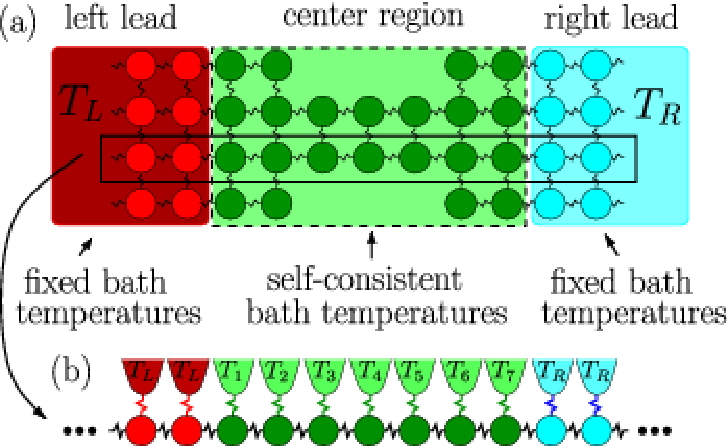
\includegraphics[width=8.6cm]{pics/pic_scbaths.pdf}
 \caption{(a) A schematic illustration of the system under study. The structure is divided into the left lead, the center region and the right lead. All atoms are coupled to spatially uncorrelated quantum Langevin heat baths, which are shown explicitly for one cross-section in (b). In the left and right lead, the temperatures of the local heat baths have prescribed values $T_L$ and $T_R$, respectively. In the center region, on the other hand, temperature varies between $T_L$ and $T_R$ and the bath temperatures are determined self-consistently using the requirement that the average thermal current to each bath vanishes. The leads can contain an infinite number of atoms, but the center region is finite. Two-dimensional square lattice with nearest neighbor interactions is shown for illustrative purposes, but the basic principle can be applied to any geometry.}
\label{fig:sud1}
\end{center}
\end{figure}

Quantum effects cannot be rigorously accounted for using molecular dynamics simulations. Therefore, one must find alternative methods to solve the equations of motion. The solution is, however, practically impossible due to the non-linear terms arising from the anharmonicity in the interatomic potential. The usual approach in traditional Landauer-B\"uttiker calculations \cite{zhang07} is to neglect the anharmonic terms, but then the model can only describe purely ballistic phonon transport. 

To account both for quantum statistical effects and non-ballistic transport, one can mimic the anharmonic terms responsible for phonon decay by an effective frictional term in the equation of motion. To be consistent with the fluctuation-dissipation theorem, the dissipative term must, however, be accompanied by a stochastic force term. The atoms are then effectively coupled to Langevin heat baths. The requirement of local current conservation leads to the requirement of solving the heat bath temperature self-consistently, leading to the self-consistent heat bath model described below. The self-consistent heat bath model was first proposed by Bolsterli, Rich, and Visscher to describe diffusive heat transfer in one-dimensional systems \cite{bolsterli70} and has since been used in multiple works investigating, e.g., the ballistic-diffusive transition in low-dimensional systems \cite{bonetto04,dhar06,roy08} and the necessary conditions for thermal rectification \cite{pereira08,segal09,bandyopadhyay11}.

The system under study is schematically illustrated in Fig. \ref{fig:sud1}. The setup resembles the classical Landauer-B\"uttiker setup \cite{datta}, consisting of the left lead region, center region and right lead region. Contrary to the Landauer-B\"uttiker setup, however, all atoms are coupled to ohmic Langevin heat baths mimicking scattering events such as phonon-phonon scattering driving the system towards local thermal equilibrium. In the leads, the bath temperatures are set to prescribed values $T_L$ and $T_R$. The atoms in the center region are coupled to local heat baths whose temperatures are determined self-consistently from the requirement of local current conservation. The presence of heat baths both in the leads and center region ensures perfect acoustic matching at the fictional interfaces separating the regions. %The coupling to the Langevin heat baths effectively .

To write down the equation of motion for the atoms, we observe that the time evolution consists of (1) the deterministic part, specified by the system Hamiltonian $\ca{H}$ and the Heisenberg equations of motion, and (2) the stochastic part due to the interaction with the heat baths.  Part (1) is specified by writing down the harmonic Hamiltonian for the system:
\begin{equation}
 \ca{H} = \frac{1}{2}  \sum_I \left[ \frac{\bb{p}_I^2}{m}+\bb{u}_I^T\bb{K}_I \bb{u}_I \right] + \sum_I \sum_{J\neq I} \bb{u}_I^T \bb{V}_{IJ} \bb{u}_J.
\end{equation}
The index $I\in\{C,L,R\}$ labels the region: $C$ stands for center region, and $L$ and $R$ for the left and right leads, respectively. For each index $I$, the atomic displacement vector $u_i^{\alpha}=r_i^{\alpha}-r_i^{\alpha 0}$ is defined as the displacement of position $r_i^{\alpha}$ from the equilibrium position $r^{\alpha 0}_i$, where $\alpha\in\{x,y,z\}$. The atomic momenta are in vectors $\bb{p}_I$. We assume the masses $m$ of all atoms to be equal. The spring constant matrix $\bb{K}_I$ and the inter-region coupling matrices $\bb{V}_{IJ}$ are the blocks of the full spring constant matrix $\bb{K}$ [Eq. \eqref{eq:th_K_def}]:
\begin{equation}
 \bb{K} = \left(\begin{matrix}
                 \bb{K}_L & \bb{V}_{LC} & 0 \\
		\bb{V}_{CL} & \bb{K}_C & \bb{V}_{CR} \\
		0 & \bb{V}_{RC} & \bb{K}_R.
                \end{matrix}
 \right)
\end{equation}
 
The Heisenberg equations of motion, which coincide with the classical equations of motion $m\ddot{\bb{u}}_I=-\partial \ca{H}/\partial \bb{u}_I$ due to the linearity of the system, can be determined from the Hamiltonian. Accompanied with the non-Hamiltonian time-evolution arising from the Ohmic interaction with the heat bath [see Eq. \eqref{eq:th_ohmic}], the equations of motion are then
\begin{equation}
  m\ddot{\bb{u}}_I = - \bb{K}_I \bb{u}_I - \sum_{J\neq I} \bb{V}_{IJ} \bb{u}_J - m \gamma \dot{\bb{u}}_I + \xi_I. \label{eq:gfm_eom_I}
\end{equation}

Our goal is to derive an explicit solution for the atomic dynamics $\bb{u}_C$, from which one can calculate the time-averages of heat currents both to the leads and to the local baths. The expression for $\bb{u}_C$ can be determined by (1) eliminating the time derivatives by temporal Fourier transform and (2) solving the equation of motion for $\bb{u}_L$ and $\bb{u}_R$ and substituting to the equation of $\bb{u}_C$. As shown in detail in \citepub{dipole}, one gets
\begin{equation}
 \hat{\bb{u}}_C(\omega) = - \bb{G}(\omega) \left[ \hat\xi_C(\omega) + \sum_{I=L,R} \hat{\eta}_I(\omega) \right]. \label{eq:gfm_uc_sol}
\end{equation}
Here the Green's function for the center region is defined as the matrix inverse
\begin{equation}
 \bb{G}(\omega) = \left[m\omega^2 - \bb{K}_C(\omega) +im\gamma(\omega) - \sum_{I=L,R} \Sigma_I(\omega)  \right]^{-1}.
\end{equation}
The coupling to the leads appears only through the lead self-energies
\begin{equation}
 \Sigma_I(\omega) = \bb{V}_{CI} \bb{g}_I(\omega) \bb{V}_{IC} \label{eq:th_sigmaI}
\end{equation}
responsible for phonon ''leak'' to the leads and the lead-coupled Langevin noise terms
\begin{equation}
 \hat\eta_I(\omega) = \bb{V}_{CI}\bb{g}_I(\omega) \hat{\xi}_I(\omega). \label{eq:th_etaI}
\end{equation}
representing the stochastic arrival of phonons from the leads to the center region. The decoupled Green's function of the leads appearing in Eqs. \eqref{eq:th_sigmaI} and \eqref{eq:th_etaI} are
\begin{equation}
 \bb{g}_I(\omega) = \left[m\omega^2+im\gamma\omega - \bb{K}_I \right]^{-1}.
\end{equation}
As shown in \citepub{gf}, the lead noise terms $\hat\eta_I(\omega)$ satisfy the fluctuation-dissipation relation analogous to Eq. \eqref{eq:th_xixiom}:
\begin{equation}
 \langle \hat\eta_I(\omega) \hat\eta_I(\omega')^T \rangle=2\pi\delta(\omega+\omega') \Gamma^I(\omega) \left[f_B(\omega,T_I)+1 \right] \label{eq:th_etaIetaI}
\end{equation}
where $\Gamma^I(\omega)=-2\textrm{Im}[\Sigma_I(\omega)]$.

Having the solution \eqref{eq:gfm_uc_sol} and the fluctuation-dissipation relations for the local heat baths [Eq. \eqref{eq:th_xixiom_ohmic_qm}] and leads [\eqref{eq:th_etaIetaI}] available, one can calculate the heat currents flowing to the local heat baths and to the leads. As shown in Publication \cp{gf}, the heat current to the local heat baths (bath index $I\in \{1,\dots,N_C\}$, $N_C$ being the number of atoms in the center region) or to the leads ($I \in \{L,R\}$) can be written in the compact form
\begin{equation}
 \langle Q_I \rangle =  \int_0^{\infty} \frac{d\omega}{2\pi} \hbar \omega \sum_{J} \ca{T}_{IJ}(\omega)[f_B(\omega,T_J)-f_B(\omega,T_I)], \label{eq:gfm_qi}
\end{equation}
where the transmission function from lead $J$ to lead $I$ is the matrix trace 
\begin{equation}
 \ca{T}_{IJ}(\omega) = \textrm{Tr}[\Gamma^I(\omega) \bb{G}(\omega) \Gamma^J(\omega) \bG(\omega)^{\dagger}]. \label{eq:gfm_caroli}
\end{equation}
The coupling functions $\Gamma^I(\omega)$ are defined as $\Gamma^i(\omega)=2m\gamma\omega \bb{I}_{3\times3}$ for the local heat baths.

Equation \eqref{eq:gfm_qi} is the multiprobe Landauer-B\"uttiker formula \cite{buttiker92} for energy transfer between heat baths. Equation \eqref{eq:gfm_caroli} was first derived for electron energy transfer by Caroli \textit{et al.} \cite{caroli71} and later derived for phonon transfer from the mode picture \cite{mingo06} and Keldysh formalism \cite{yamamoto06}. In Publication \cp{gf}, we derived the formula using local Langevin heat baths and thereby also included dissipative effects in the leads.

As mentioned above, the bath temperatures in the center region must be determined self-consistently from the requirement of vanishing energy current (Eq. \eqref{eq:gfm_qi}] to the baths. Because the bath temperatures $T_i$ appear in the Bose-Einstein function in the expression for the current, one must solve a non-linear system of equations. The solution to the system of equations can be determined exactly by using, e.g., the Newton-Raphson method \cite{bandyopadhyay11} or approximately by linearizing the equations in terms of temperatures \cite{segal09}. In \citepub{gf}, we compared the exact and linearized solutions and also suggested an alternative method for solving the equations, based on considering the transient time evolution of bath temperatures and integrating the time evolution equations until steady-state is achieved. 

%\textbf{Solution of self-consistent equations}

\subsection{Fluctuating dipole model}

\label{sec:em_methods}

\begin{figure}
 %\includegraphics[width=15.6cm]{pic1.ps}
%  \includegraphics[width=.49\columnwidth]{../dipole_resubmission/pic1a}
 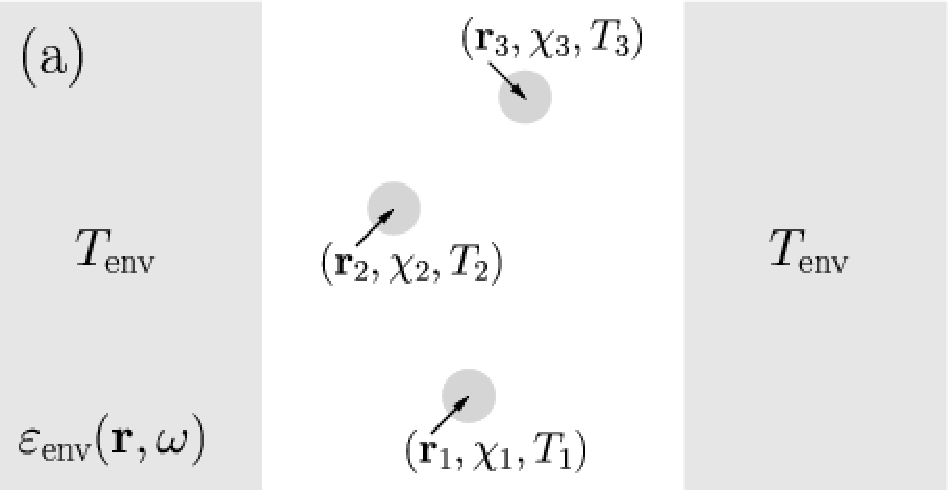
\includegraphics[width=.49\columnwidth]{pics/dipole_pic1a.pdf}
 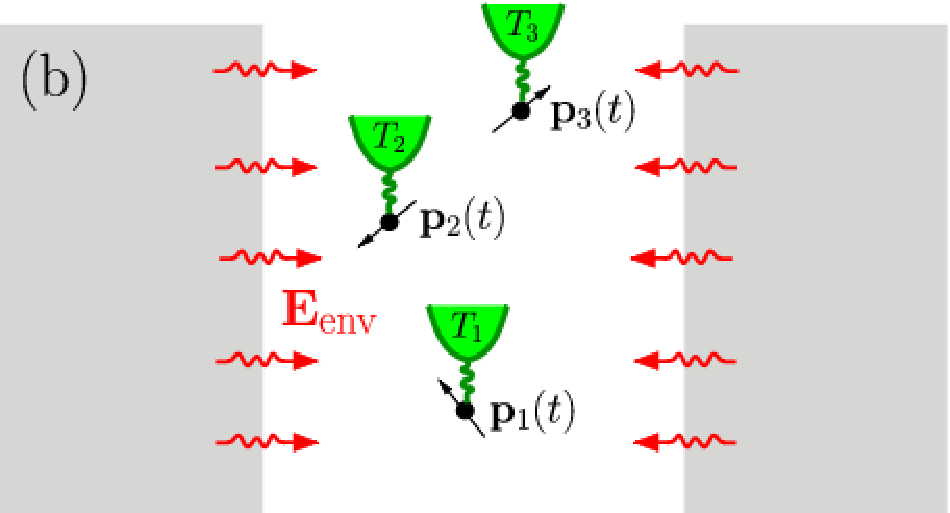
\includegraphics[width=.49\columnwidth]{pics/dipole_pic1b.pdf}
%   \includegraphics[width=.49\columnwidth]{../dipole_resubmission/pic1b}
 \caption{(a) A schematic illustration of the studied electromagnetic energy transfer setup. A collection of dielectric particles with positions $\mathbf{r}_i$, $i\in\{1,\dots,N\}$, electric susceptibilities $\chi_i(\omega)$ and temperatures $T_i$ is located in an inhomogeneous environment, consisting in the shown case of two dielectric (or metallic) bodies forming a cavity. The overall relative permittivity is $\varepsilon(\br,\omega)=\epsenv(\br,\omega)$ outside the particles and $\varepsilon(\br_i,\omega)=1+\chi_i(\omega)$ at the position of each particle coordinate $\br_i$. The two cavity walls, described by the environment dielectric constans, are assumed to act as a source of thermal radiation at temperature $\Tenv$. The polarization field inside each particle $i$ is modeled as an oscillating point dipole moment $\bb{p}_i$ coupled to a local Langevin heat bath at temperature $T_i$ as depicted in (b). The total local field $\bE(\br_i,t)$ driving each dipole moment $\bb{p}_i$ is the sum of the stochastic background field $\bE_{\textrm{env}}(\br_i,t)$ and the fields $\bE_{ij}(t)$ created by each dipole $j$.}%The local bath temperatures $T_i$ correspond to local lattice temperatures, which could either by given fixed temperatures or could be self-consistently determined by the balance of absorption, emission and the in- and outflow of lattice heat. 
\label{fig:gfm_dipole_system}
\end{figure}

This section is devoted to the theory of electromagnetic energy transfer developed in detail in \citepub{dipole}. As discussed in Sec. \ref{sec:intro_emtheory}, we have developed a more microscopic alternative to fluctuational electrodynamics, which is traditionally used to describe electromagnetic energy transfer \cite{joulain05}. Although our final expressions for energy transfer rates are fully equivalent to fluctuational electrodynamics results (see, e.g., Ref. \cite{messina13}), our theory more transparently treats the radiation damping, straightforwardly allows for deriving expressions for heat transfer rates in terms of various different definitions of the local polarizability and allows for coupling the optical degrees of freedom to other degrees of freedom such as acoustic phonons.

We briefly outline our quantum Langevin equation approach to the electromagnetic energy transfer here. More details are found in \citepub{dipole}. The studied system is depicted in Fig. \ref{fig:gfm_dipole_system}. Dielectric particles with positions $\mathbf{r}_i$, $i\in\{1,\dots,N\}$ are located in an inhomogeneous environment characterized by the environment's dielectric constant $\epsenv(\br,\omega)$. For inhomogeneous $\epsenv(\br,\omega)$, the environment acts not only as a source of non-blackbody thermal radiation (at temperature $\Tenv$) but also as a scatterer of the radiation emitted by the particles, thereby modifying the energy transfer rates compared to the free space. The overall relative permittivity is given by $\varepsilon(\br_i,\omega)=1+\chi_i(\omega)$ at the locations of the particles ($\chi_i$ being the electric susceptibility of particle $i$) and $\varepsilon(\br_i,\omega)=\epsenv(\bb{r},\omega)$ elsewhere. The microscopic dipole moments, which represent the fluctuating electric polarization inside each particle, are oupled to (1) local heat baths describing thermal fluctuations and dissipation, (2) to the electromagnetic field arising from other dipoles, and (3) to the thermal field originating from the environment. Following the dipole approximation \cite{novotny}, we assume each particle to be smaller than the optical wavelength so that we can treat the particles as dipoles located at locations $\br_i$, but the theory can be straightforwardly generalized to larger particles as well by dividing the particles into small dipolar volumes as in the traditional discrete dipole method \cite{novotny}. 

%Following the dipole approximation, the internal polarization field of each particle is modeled as a point dipole located at the central coordinate $\br_i$ of the particle $i$ as illustrated in Fig. \ref{fig:sud1}(b). 

\subsubsection{Equation of motion and solution}

The local dynamics of each dipole is modeled by the classical oscillator model accompanied by quantum Langevin dynamics. The equation of motion for the local dipole displacement $\bu_i$, related to the dipole moment through $\bp_i=\bu_i/q$ where $q$ is the charge, reads
 \begin{equation}
 m\ddot\bu_i(t) = -m\omega_i^2 \bu_i(t) +\xi_i(t) -m\gamma_i \dot{\bu}_i(t)  + q \bE_i(t). \label{eq:gfm_eom1}
\end{equation}
The oscillator mass $m$, charge $q$, resonance frequency $\omega_i$ and the friction parameter $\gamma_i$ are absorbed into the definition of the local polarizability in the final expressions. The stochastic force $\xi_i(t)$, which is related to the friction term $m\gamma_i\dot{\bu}_i(t)$ by the standard fluctuation-dissipation relation \eqref{eq:th_xixiom_ohmic_qm}, accounts for thermal fluctuations. 

The steady state solution to the equations of motion can be most easily achieved by moving to frequency domain, in which the equations of motion become
\begin{equation}
 -m\omega^2 \hat\bu_i(\omega) = -m\omega_i^2 \hat\bu_i(\omega) +\hat \xi_i(\omega) +im\gamma_i \omega \hat \bu_i(\omega)  + q \hat \bE_i(\omega). \label{eq:gfm_eom2}
\end{equation}
Here, the Fourier transform of the local electric field $\hat \bE_i$ consists of the environment field $\Eenvhat(\br_i,\omega)$ and the fields $\hat \bE_{ij}(\omega)$ generated by each dipole $j$ [Eq. \eqref{eq:th_Etilde} with spatially localized sources]:
\begin{equation}
 \hat{\bE}_i\pom= \Eenvhat(\br_i,\omega) + \sum_{j=1}^N \hat{\bE}_{ij}\pom. \label{eq:gfm_etot}
\end{equation}
The electric field $\bE_{ij}$ due to dipole moment $\hat{\bb{p}}_j$, responsible for the electromagnetic interaction between the dipoles, is given in frequency domain by [Eq. \eqref{eq:th_Etilde}]
\begin{equation}
 \hat{\bE}_{ij}(\omega) = \omega^2 \mu_0\gem_{ij}(\omega) \hat{\bp}_j (\omega), \label{eq:gfm_ekl}
\end{equation}
where $\gem_{ij}(\omega)\equiv \gem(\br_i,\br_j;\omega)$ is found from Eq. \eqref{eq:intro_gemdef} for given $\epsenv(\br,\omega)$. The stochastic environment field has zero average and satisfies the fluctuation-dissipation relation \cite{novotny}
\begin{alignat}{2}
  q^2 \langle \Eenvhat(\bb{r}_i,\omega) \Eenvhat(\bb{r}_j,\omega')^T \rangle   &=  2\pi \delta(\omega+\omega') \hbar \Gamma^{\textrm{rad}}_{ij}(\omega) \fbbg, \label{eq:gfm_ebgebg1}
\end{alignat}
where the coupling function of the dipoles to the radiation field is
\begin{equation}
 \Gamma_{ij}^{\textrm{rad}}(\omega) = 2 q^2\omega^2\mu_0 \textrm{Im}[\gem_{ij}(\omega)]. \label{eq:gfm_gammarad_def}
\end{equation}

It is important to stress that while the Green's dyadic $\gem$ only accounts for the scattering of the electromagnetic field from the inhomogeneities in the environment, the scattering of the field from the point dipoles is automatically included in the formalism by the coupled dipole equations of motion. The local Green's dyadic $\gem_{ii}(\omega)$, discussed in more detail in \citepub{dipole}, accounts for the Abraham-Lorentz radiation damping, which produces a force term proportional to third time derivative of $\bb{u}$ in the dipole equation of motion \eqref{eq:gfm_eom1}. The fluctuations accompanying the radiation reaction damping are responsible for generating thermal radiation \cite{greffet10}.

The substitution of Eqs. \eqref{eq:gfm_etot} and \eqref{eq:gfm_ekl} to Eq. \eqref{eq:gfm_eom2} gives
\begin{equation}
 -m\omega^2 \hat{\bu}_i \pom =  -m\omega_i^2 \hat \bu_i\pom + \hat{\xi}_i\pom + im\gamma_i \omega \hat{\bu}_i\pom + \Eenvhat(\br_i,\omega) + q^2\omega^2\mu_0 \sum_{j=1}^N \gem_{ij}\pom \hat{\bu}_j\pom. \label{eq:gfm_eom_freq}
\end{equation}
Equation \eqref{eq:gfm_eom_freq} can be rearranged as
\begin{equation}
 - \sum_{j} \bb{A}_{ij} \hat{\bu}_j(\omega) = \hat{\xi}_i(\omega) + q\Eenvhat(\br_i,\omega) \label{eq:gfm_eom_akl}
\end{equation}
by defining an inverse propagator
\begin{equation}
 \bb{A}_{ij} = \left[m(\omega^2-\omega_i^2+i\gamma_i) \right]\delta_{ij}\bb{I}_{3\times 3}+ q^2\omega^2\mu_0 \gem_{ij},
\end{equation}
where $\unitdyadic$ is the $3\times 3$ unit matrix. The solution to Eq. \eqref{eq:gfm_eom_akl} can be written compactly in matrix form as
\begin{equation}
 \hat{\bu}(\omega) = -\bb{G}(\omega) \left[\hat{\xi}(\omega)+q\Eenvhat(\omega) \right], \label{eq:gfm_usol}
\end{equation}
where the dipole displacement Green's function $\bb{G}\pom=\bb{A}\pom^{-1}$ is
\begin{equation}
 \bb{G}(\omega) = \frac{1}{m(\omega^2 \mathbf{I}_{3N\times 3N}-\Omega^2)+q^2\omega^2\mu_0 \textrm{Re}[\gem(\omega)]+i\Gamma^{\textrm{bath}}(\omega)/2+i\Gamma^{\textrm{rad}}(\omega)/2}. \label{eq:gfm_g_expression1}
\end{equation}
Here we adopted a matrix notation where the dipole indices $i\in \{1,\dots,N\}$ and the spatial components $\alpha\in \{1,2,3\}$ are combined into a composite index resulting in matrices and vectors of size $3N\times 3N$ and $3N$, respectively. In the following, we will use an index notation where the subscript $ij$ ($i$) always refers to the $3\times 3$ matrix (3-component vector) corresponding to the notation used before Eq. \eqref{eq:gfm_usol}.

In Eq. \eqref{eq:gfm_usol}, we have additionally defined the block-diagonal resonance frequency matrix as $\Omega=\textrm{diag}(\omega_1\bb{I}_{3\times 3},\omega_2\bb{I}_{3\times 3},\dots,\omega_N\bb{I}_{3\times 3})$ and the block-diagonal bath coupling matrix as $\Gamma^{\textrm{bath}} (\omega) = \textrm{diag}(2m \gamma_1 \omega\bb{I}_{3\times 3},\dots,2m\gamma_N \omega_N \bb{I}_{3\times 3})$.

%In the denominator of Eq. \eqref{eq:g_expression1} and in all matrix-valued expressions appearing below, the scalar terms should be interpreted as being proportional to the unit matrix of size $3N\times3N$.

Equation \eqref{eq:gfm_g_expression1} shows that both the coupling to heat baths and the coupling to the radiation field produce broadening in the Green's function via the coupling functions $\Gamma^{\textrm{bath}}(\omega)$ and $\Gamma^{\textrm{rad}}(\omega)$. This broadening in the Green's function reflects dissipation that, along with the accompanying thermal fluctuations, enables energy transfer between dipoles with different bath temperatures.

\subsubsection{Heat current}

The heat transfer rates between particles could in general be calculated from the electromagnetic Poynting vector, but the calculations can be simplified by energy conservation arguments. A direct calculation shows that the expectation value of the Poynting vector's flux across a surface $\partial V_i$ enclosing a particle $i$, equal to the power of the emitted radiation field, satisfies 
\begin{equation}
 \left\langle \int_{\partial V_i} \bb{S} \cdot d\bb{S} \right\rangle = - \langle Q_i \rangle,
\end{equation}
where the energy current to the bath is given by the bath force multiplied by the dipole moment ''velocity'': $Q_i = (m\gamma \dot{\bu}_i-\xi_i)\cdot \dot{\bu}_i$. Therefore, $\langle Q_i\rangle$ can be interpreted as the locally absorbed power. Direct calculation carried out in \citepub{dipole} shows that 
\begin{alignat}{2}
 \langle Q_i \rangle &= \int_0^{\infty}\frac{d\omega}{2\pi} \hbar\omega \sum_{j} \ca{T}_{ij}(\omega) \left[f_B(\omega,T_j)-f_B(\omega,T_i ) \right] \notag \\
  & \quad + \int_0^{\infty} \frac{d\omega}{2\pi} \hbar \omega \ca{T}_{i,\textrm{rad}}(\omega)\left[ f_B(\omega,\Tenv)-f_B(\omega,T_i)\right].
\end{alignat}
Here the dipole-dipole transmission function is defined as
\begin{equation}
 \ca{T}_{ij}(\omega) = \textrm{Tr} \left[\Gamma_i(\omega) \bb{G}(\omega) \Gamma_j(\omega) \bb{G}(\omega)^{\dagger} \right]
\end{equation}
and the dipole-environment transmission is 
\begin{equation}
 \ca{T}_{i,\textrm{rad}}(\omega) =  \textrm{Tr} \left\{ \Gamma_i(\omega) \left[ \bb{G}(\omega) \Gamma_{\textrm{rad}}(\omega) \bb{G}(\omega)^{\dagger} \right]_{ii} \right\}. \label{eq:th_Tirad}
\end{equation}

\subsubsection{Local polarizabilities}

To calculate the transmission functions, it is useful to express the transmission function in terms of purely optical quantities. This can be achieved by (i) absorbing the microscopic, auxiliary parameters $m$, $q$, $\gamma_i$ to the definitions of the local polarizabilities and (ii) expressing the Green's function in terms of the electromagnetic Green's dyadics. For (i), one must specify the microscopic definition for the polarizability. While there are at least three different definitions available, we use here the Clausius-Mossotti definition 
\begin{equation}
 \langle \hat \bp_i(\omega) \rangle = \varepsilon_0 \alpha_{\textrm{CM}}^i(\omega) \left[\hat \bE_0(\br_i,\omega)+ \left\langle \hat \bE_{\textrm{pol},i} (\omega) \right\rangle \right]
\end{equation}
relating the expectation value of the local dipole moment to the sum of the external field $\bE_0(\br_i,\omega)$ and the polarization field $\bE_{\textrm{pol},i} (\omega)=\hat \bp_i(\omega) /(3\varepsilon_0 \Delta V_i)$ ($\Delta V_i$ is the particle volume). By solving the equation of motion for a single dipole in an external field, one gets 
\begin{equation}
 \alpha_{\textrm{CM}}^i(\omega) = - \frac{q^2}{\varepsilon_0} \frac{1}{m(\omega^2-\omega_i^2+i\gamma_i)-q^2/(3\varepsilon_0\Delta V_i)}\unitdyadic. \label{eq:gfm_alpha_cm_expr}
\end{equation}
One can also start from the microscopic definitions $\varepsilon_i(\omega)=1+\chi_i(\omega)$, $\hat{\bb{P}}(\bb{r}_i,\omega)=\varepsilon_0 \chi_i(\omega) \hat{\bb{E}}(\bb{r}_i,\omega)$ and $\hat{\bb{P}}(\bb{r}_i,\omega)=\hat{\bb{p}}_i(\omega)/\Delta V_i$ to show that
\begin{equation}
 \alpha_{\textrm{CM}}^i(\omega) = 3\Delta V_i \frac{\varepsilon_i(\omega)-1}{\varepsilon_i(\omega)+2} \unitdyadic. \label{eq:gfm_alphacm_epsilon}
\end{equation}
Equations \eqref{eq:gfm_alpha_cm_expr} and \eqref{eq:gfm_alphacm_epsilon} provide the link between the microscopic parameters and the macroscopic dielectric constant $\varepsilon_i(\omega)$ of the particle $i$.

Using Eq. \eqref{eq:gfm_alpha_cm_expr} and straightforward albeit tedious algebraic manipulations, one can write the dipole-dipole energy transmission function as
\begin{equation}
   \ca{T}_{ij}(\omega) = 4 \kw^4 \textrm{Tr} \left[ \textrm{Im}[\alpha^i_{\textrm{CM}}(\omega)] \gemfull_{ij}\pom \textrm{Im}[\alpha^j_{\textrm{CM}}(\omega)] \gemfull_{ji}(\omega)^{\dagger}\right]. \label{eq:tij_final}
\end{equation}
Here the electromagnetic Green's dyadic $\gemfull(\omega)$ expressed in terms of the Clausius-Mossotti polarizabilities of the particles has been defined as 
\begin{alignat}{2}
 \gemfull(\omega) &= \frac{1}{\kw^2} \left[\frac{1}{1-\kw^2 \gem(\omega)\alpha_{\textrm{CM}}(\omega)}\right] \alpha_{\textrm{CM}}(\omega)^{-1} \\
  &\equiv \frac{1}{\kw^2} \alpha_{\textrm{CM}}(\omega)^{-1} + \underbrace{ \left[\frac{1}{1-\kw^2 \gem(\omega)\alpha_{\textrm{CM}}(\omega)} \right] \gem(\omega)}_{\tildegemfull}. \label{eq:gfm_gemmb_cm_app}
\end{alignat}
The first term of Eq. \eqref{eq:gfm_gemmb_cm_app} is local and does not contribute to dipole-dipole energy transfer. The second term of Eq. \eqref{eq:gfm_gemmb_cm_app}, denoted by $\tildegemfull$, is non-local and therefore responsible for dipole-dipole energy transfer. By comparing the expression \eqref{eq:gfm_gemmb_cm_app} to the one obtained from FED \cite{benabdallah11}, one can show that $\tildegemfull$ is readily interpreted as the electromagnetic Green's dyadic that fully incorporates the scattering caused by the dipoles. %In our manuscript, Eq. \eqref{eq:gfm_gemmb_cm_app} arises as a convenient definition that allows us to express the transmission function \eqref{eq:tij_final} in terms of purely optical quantities.

The radiation transmission function \eqref{eq:th_Tirad} can be similarly written in terms of the polarizabilities and the Clausius-Mossotti Green's dyadic as
\begin{alignat}{2}
 \ca{T}_{i,\textrm{rad}}(\omega) 
 &= 4 \kw^6 \sum_{j,k=1}^N \textrm{Tr}\left\{   \textrm{Im}[\alpha^i_{\textrm{CM}}(\omega)] \gemfull_{ij}(\omega) \alpha_{\textrm{CM}}^j(\omega) \textrm{Im}[\gem_{jk}(\omega)] \alpha^k_{\textrm{CM}}(\omega)^* \gemfull_{ki}(\omega)^{\dagger} \right\}. \label{eq:tirad_final}
\end{alignat}
An equation similar to \eqref{eq:tirad_final} was derived very recently before the publication of Publication \cp{dipole} by Messina \textit{et al.} \cite{messina13}.


\subsection{Self-consistent electron bath model}
